
%-----------------------------------------------------------------------------
% Chapter: Development
%-----------------------------------------------------------------------------

\chapter{Development}
\label{chap:DEV}

\section{Methodology}
The most important point in the development process of the \emph{Course2018}
LMS is the idea of \emph{continuous integration} (CI), meaning that every
newly-developed feature is tested and integrated to the existing server seamlessly.

\medskip
This is achieved by using a development tool called \emph{GitLab CI}
\cite{BgitlabCI}, a sub-system that came with the source management tool,
\emph{GitLab}~\cite{Agitlab}, which is also used for the development of this
project. 

\medskip

This tool chain offers abilities to a developer so that every time
the developer finishes the programming of a feature and pushes the code to the
\emph{GitLab} project repository, the \emph{GitLab} server automatically
invokes some
routines to test the new code with a test scheme also defined by the developer
prior to the time when the code was pushed. If all tests are passed, 
the \emph{GitLab} server then deploys the new version of the project by simply
building a new container with the latest code, and has the old
container replaced with the new one. 

\section{Deployment}
In the development process of this project, the deployment stage was defined
before the actual programming even begun. This approach makes sure that all
modules of the project can be tested in the
deployment environment (i.e., the container in which the \emph{Course2018}
will be eventually running) as soon as the implementation if finished.

\subsection{Environment}
The \emph{Course2018} LMS is containerized in an environment
(the production container) based on
\emph{Debian 8}~\cite{debian}, with \emph{Python 3} and all necessary packages
(including \emph{Django 2.0}) installed.

\subsection{HTTP server}
An \emph{HTTP server} is included in the production container to host the
\emph{Course2018} LMS.
The \emph{HTTP server} in use in the production container is the
\emph{Apache HTTP server} (version 2.4)~\cite{apache}, with the
\texttt{mod\_wsgi}~\cite{wsgi} package installed to accommodate
\emph{Python} web applications in the \emph{WSGI}
(Web Server Gateway Interface~\cite{wsgi}) specification, such as a
\emph{Django} project.

\section{System development}

\subsection{MVT}
\label{sec:MVT}
The \emph{Django} framework enforces developers to apply an architectural
pattern called the \emph{MVT} (Model-View-Template) pattern to their projects.
In such projects,
all data models are defined as \texttt{Model} classes, which
then are used to create schemas for corresponding database tables.
The data in the data models will then be retrieved and organized in 
methods of different \texttt{View} classes, each of which 
is connected to a \emph{URL};
webpages will finally be generated by those \texttt{View} classes
using different \emph{HTML} \texttt{Templates} with the organized data.

\subsection{APIs}
In the \emph{Course2018} LMS, some views are not paired with templates, and
they do not return webpages to the users.
Instead, they return some
\emph{JSON}-formatted data.
These views are the application programming interfaces (APIs) of the system,
and they are used for updating information in
a loaded page dynamically with \emph{AJAX}~\cite{AJAX}. 


%-----------------------------------------------------------------------------
% Section: User authentication
%-----------------------------------------------------------------------------

\subsection{User authentication}
As discussed in Section~\ref{sec:USRAUTH}, user authentication is handled by the
\emph{Django User Model} provided by the \emph{Django} \texttt{auth} library.
Not only does this approach simplify the implementation of the module,
but in addition security is also improved in comparison with implementing the authentication
module solely by the developer.

\subsubsection{Data model}
The data model of the user authentication module is shown in
Figure~\ref{fig:AUTH_ER}, Table~\ref{tab:USR_ATTR} and
Table~\ref{tab:PROFILE_ATTR}.

\bigskip

\begin{figure}[ht]
    \centering

    \usetikzlibrary{er}
    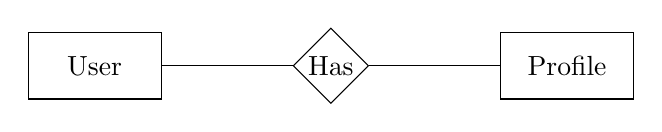
\begin{tikzpicture}[node distance = 3cm]
        \node[entity] (user) {User};
        \node[relationship] (has) [right of=user] {Has} edge (user);
        \node[entity] (profile) [right of=has] {Profile} edge (has);
    \end{tikzpicture}

    \caption{Data model of the user authentication module}
    \label{fig:AUTH_ER}
\end{figure}


\begin{table}[ht]
    \centering
    \caption{Attributes of \texttt{User} model}
    \label{tab:USR_ATTR}
    \renewcommand{\arraystretch}{1.3}
    \begin{tabular}[ht]{r|l}
        \hline
        Attribute & Note \\
        \hline
        \hline
        \texttt{id} & primary key \\
        \hline
        \texttt{username} &  required, max length: 150 \\
        \hline
        \texttt{first\_name} &  optional, max length: 30 \\
        \hline
        \texttt{last\_name} &  optional, max length: 150 \\
        \hline
        \texttt{email} & optional\\
        \hline
        \texttt{password} & A hash of the user's password \\
        \hline
        \texttt{is\_active} & \texttt{boolean field}, indicating whether or not the user
            is active \\
        \hline
        \texttt{last\_login} & \texttt{datetime field}, last login time \\
        \hline
        \texttt{date\_joined} & \texttt{datetime field}, time when the account is created \\
        \hline
    \end{tabular}
    \renewcommand{\arraystretch}{1}
\end{table}

\begin{table}[ht]
    \centering
    \caption{Attributes of \texttt{Profile} model}
    \label{tab:PROFILE_ATTR}
    \renewcommand{\arraystretch}{1.3}
    \begin{tabular}[ht]{r|p{4.5in}}
        \hline
        Attribute & Note \\
        \hline
        \hline
        \texttt{user\_id} & foreign key to a \texttt{User} model instance \\
        \hline
        \texttt{role} & \texttt{integer field}, choice from 0 and 1, indicating the
            user's role \\
           & is \emph{Student} or \emph{Professor} respectively \\
        \hline
    \end{tabular}
    \renewcommand{\arraystretch}{1}
\end{table}


\subsubsection{Views}

\begin{itemize}
    \item Login: \\
        A \texttt{UserLogin} view is defined to provide routines to handle user
        authentication, by invoking the built-in \emph{Django} library
        function~\texttt{authenticate()}
        to compare the credentials provided
        by the user against the user account database.

    \item Permission control: \\
        An abstract view class called \texttt{AbstractLoginRequiredView} is
        defined for general permission control. This class contains a function
        to check whether or not a user is authenticated. If the user is
        authenticated, the function then checks the role of the user and
        invokes \texttt{student\_view()} or \texttt{professor\_view()} to
        provide different content according to the user's role.

        All the views of the modules that require permission control are
        inherited from the \texttt{AbstractLoginRequiredView} class, and have
        the class function \texttt{student\_\-view()} and
        \texttt{professor\_view()} overridden to provide module-specific
        content for students and instructors respectively.

        In addition, there is also another abstract view class,
        \texttt{AbstractAPI}, this class provides permission
        control for all the APIs in the same manner as discussed above.
\end{itemize}

\subsubsection{Templates}

\begin{itemize}
    \item Login template: \\
        This template is used by the \texttt{UserLogin} view to provide a very
        simple login interface to the users. It contains a form with two
        fields (username and password) and a \emph{Login} button. Users can
        use this interface to log into the \emph{Course2018} LMS.
\end{itemize}


%-----------------------------------------------------------------------------
% Section: Course management
%-----------------------------------------------------------------------------

\subsection{Course management}
To provide source code management for programming assignments,
a great open-source version control tool,
\emph{Git}, is integrated into the \emph{Course2018} LMS.
\emph{Git} was originally developed by \emph{Linus Torvalds}~\cite{git},
creator and principal developer of the \emph{Linux} operating system
kernel~\cite{lTorvalds}.
Moreover, 
an open-source \emph{Git}-repository manager, \emph{GitLab}~\cite{Agitlab}, is also
used in the \emph{Course2018} LMS to enhance the source code management user
experience.

\medskip
Once an instructor enables source code management for an assignment, a remote
\emph{GitLab} repository is also created for the course to which the assignment
belongs. The name of the repository will be saved in the course management
module.


\subsubsection{Data model}
The data model of the course management module is shown in
Figure~\ref{fig:COURSE_ER} and Table~\ref{tab:COURSE_ATTR}. \bigskip

\begin{figure}[ht]
    \centering

    \usetikzlibrary{er}
    \begin{tikzpicture}[scale=0.8, every node/.style={scale=0.8}, node distance = 4cm]
        \node[entity] (course) {Course};

        \node[relationship] (stu_reg) [below of=course] {Student} edge[total] (course);
        \node[entity] (stu) [left of = stu_reg] {User (Role: student)} edge[total] (stu_reg);

        \node[relationship] (instructor) [above of = course] {Instructor} edge[total] (course);
        \node[entity] (prof) [left of = instructor] {User (Role: professor)} edge (instructor);

        \node[relationship] (ta_reg) [right of = course] {TA} edge[total] (course);
        \node[entity] (ta) [right of = ta_reg] {User} edge[total] (ta_reg);
    \end{tikzpicture}

    \caption{Data model of the course management module}
    \label{fig:COURSE_ER}
\end{figure}

\begin{table}[h]
    \centering
    \caption{Attributes of \texttt{Course} model}
    \label{tab:COURSE_ATTR}
    \renewcommand{\arraystretch}{1.3}
    \begin{tabular}[ht]{r|p{4in}}
        \hline
        Attribute & Note \\
        \hline
        \hline
        \texttt{id} & primary key \\
        \hline
        \texttt{department} & required, department code of the course
            (e.g., COMP, MATH) \\
        \hline
        \texttt{number} & required, course number \\
        \hline
        \texttt{section} & required, course section (e.g., X1) \\
        \hline
        \texttt{title} & require, course title \\
        \hline
        \texttt{semester} & required, semester of the course
            (e.g., Winter, Fall) \\
        \hline
        \texttt{year} & required, academic year of the semester \\
        \hline
        \texttt{start\_time} & required, \texttt{date} field, date the course
            becomes available to  students \\
        \hline
        \texttt{end\_time} & required, \texttt{date} field, date the course
            ends \\
        \hline
        \texttt{visible\_after\_end} & required, \texttt{boolean} field,
            indicating whether or not to allow students to access the course
            after it ends \\
        \hline
        \hline

        \texttt{instructor} & foreign key to the instructor \\
        \hline
        \texttt{students} & many-to-many relationship to the students
            registered in the course\\
        \hline
        \texttt{TAs} & many-to-many relationship to the TAs registered in the
            course \\

        \hline
        \hline

        \texttt{repo\_name} & optional, the name of the remote \emph{GitLab}
            repository  in 
            which programming assignment source code files  are stored \\
        \hline
        \hline

        \texttt{constraints} & 
            \vspace{-7mm}
            \begin{enumerate}[leftmargin=5mm]
                \item the combination of fields \texttt{department},
                        \texttt{number},
                        \hspace{2em}\texttt{section},
                        \texttt{year},
                        \texttt{semester} must be unique
                \item role of the \texttt{instructor} must be \emph{Professor}
                \item role of the each of the \texttt{students} must be
                        \emph{Student}
            \end{enumerate} \vspace{-9mm}\\
        \hline
    \end{tabular}
    \renewcommand{\arraystretch}{1}
    
\end{table}

\subsubsection{Views}

\begin{itemize}
    \label{item:NEW_COURSE}
    \item Create course: \\
        This activity is handled with the \texttt{CreateCourseView}, which is
        inherited from the \texttt{AbstractLoginRequiredView}, and is
        only accessible by instructors. 
        This view accepts all the \emph{create course} requests, validates the
        data in each of the requests, and if the data has no errors,
        creates course records with the data in the course database table.
        The permission control of this view
        (and any other views that are only accessible by instructors) is
        achieved by simply raising an \texttt{HTTPForbidden}~\citep[Section 6.5.3]{http}
        error in the overridden \texttt{student\_view()} class function.
    
    \item View course summary:\\
    When a user sends a \emph{view course} request to the server, the request
    is handled with a \texttt{CourseSummaryView} class which is inherited from
    the \texttt{AbstractLogin\-Required\-View} class.
    \begin{itemize}
        \item \texttt{student\_view()}: 
            information about the course and a list of assignments
            are fetched from the database and displayed to the registered
            students.
        \item \texttt{professor\_view()}:
            in addition to the course information,
            this function also fetches the latest student and TA activities 
            (i.e., assignment submission activities and  assignment grading
            activities),
            and calculates the latest assignment's proportion of the student
            grades.
    \end{itemize}
\end{itemize}

\subsubsection{Templates}
\begin{itemize}
    \item Create course template: \\
        This template is used by the \texttt{CreateCourseView}; the template
        contains a form to be filled out by the user who
        wishes to create a course. 
    \item Course summary template:
    \begin{itemize}
        \item Student template: a web page with the course information
            (e.g., department, number, section, and title)
            displayed as the page title, and a list of assignments displayed
            in a table.
        \item Professor template: the same page title displayed with the course
            information as in the student template;
            the page content is divided into three sections:
            \begin{enumerate}
                \item Manage area, where an instructor can add and remove
                    students, TAs, and assignments.
                \item Latest assignment statistics area, where the latest
                    assignment's student grades proportion is displayed
                    in a horizontal bar chart.
                \item Latest activities area, where the latest TA and student
                    activities are displayed in tables.
            \end{enumerate}
    \end{itemize}
\end{itemize}

\FloatBarrier




%-----------------------------------------------------------------------------
% Section: Assignment management
%-----------------------------------------------------------------------------

\subsection{Assignment management}
\label{sec:ASM_MAN}

\subsubsection{Data model}
The data model of the assignment module module is shown in
Figure~\ref{fig:ASM_ER}, Table~\ref{tab:ASM_ATTR},
and Table~\ref{tab:COMMIT_ATTR}. \bigskip

\begin{figure}[ht]
    \centering

    \usetikzlibrary{er}

    \begin{tikzpicture}[scale=0.8, every node/.style={scale=0.8}, node distance = 4cm]
        \node[entity] (course) {Course};

        \node[relationship] (course_asm) [below of =course] {has} edge (course);
        \node[entity] (asm) [below of = course_asm] {Assignment} edge[total] (course_asm);

        \node[relationship] (asm_commit) [below of = asm] {has} edge (asm);
        \node[entity] (commit) [below of = asm_commit] {Commit} edge[total] (asm_commit);

        \node[relationship] (ta_grade) [right of = commit] {grades} edge[total] (commit);
        \node[entity] (ta) [right of = asm] {User (TA)} edge (ta_grade) edge (ta_grade);

        \node[relationship] (commit_stu) [left of = commit] {creates} edge (commit);
        \node[entity] (stu) [left of = asm] {User (Student)} edge (commit_stu);

    \end{tikzpicture}

    \caption{Data model of the assignment management module}
    \label{fig:ASM_ER}
\end{figure}

\begin{table}[ht]
    \centering
    \caption{Attributes of \texttt{Assignment} model}
    \label{tab:ASM_ATTR}
    \renewcommand{\arraystretch}{1.3}
    \begin{tabular}[ht]{r|p{4in}}
        \hline
        Attribute & Note \\
        \hline
        \hline

        \texttt{id} & primary key \\
        \hline
        \texttt{course} & foreign key to the course to which the assignment
            belongs \\
        \hline
        \hline

        \texttt{title} & required, title of the assignment\\
        \hline
        \texttt{assignment\_number} & required, number of the assignment\\
        \hline
        \texttt{description} & required, description of the assignment 
            in \emph{HTML} format \\
        \hline
        \texttt{num\_of\_problems} & required, default: 1 \\
        \hline
        \texttt{total\_grade} & required, total grade of each problem \\
        \hline
        \texttt{due} & required, time the assignment is due, default: 7:00 PM,
            seven days  from the time when the assignment is created \\
        \hline
        \texttt{is\_released} & \texttt{boolean} field, indicating whether or not
            students can view the grade and feedback \\
        \hline
        \texttt{created\_time} & time when the assignment is created \\
        \hline
        \texttt{modified\_time} & time of the last modification of an assignment
            object\\
        \hline
        \texttt{attachment\_path} & path to the directory where the attachments
            are saved \\
        \hline
        \hline

        \texttt{use\_git} & \texttt{boolean} field, indicating whether or not
            the  assignment uses \emph{Git} to provide source code management \\
        \hline
        \texttt{auto\_run} & \texttt{boolean} field, indicating whether or not
            automated test  is enabled \\
        \hline
        \hline

        \texttt{constraints} & the combination of \texttt{course} and \texttt{assignment\_number}
            must  be unique \\
        \hline
    \end{tabular}
    \renewcommand{\arraystretch}{1}
\end{table}

\begin{table}[ht]
    \centering
    \caption{Attributes of \texttt{Commit} model}
    \label{tab:COMMIT_ATTR}
    \renewcommand{\arraystretch}{1.3}
    \begin{tabular}[ht]{r|p{4in}}
        \hline
        Attribute & Note \\
        \hline
        \hline

        \texttt{id} & primary key \\
        \hline
        \texttt{assignment} & foreign key to the assignment to which a commit
            instance belong \\
        \hline
        \texttt{by} & foreign key to the student who created the commit \\
        \hline
        \hline

        \texttt{problem} & required, indicating to which problem a student's
            submission pertains \\
        \hline
        \texttt{file\_path} & required, path to the directory where files that
            the student  submits are stored \\
        \hline
        \texttt{commit\_time} & time when a commit instance is created \\
        \hline
        \texttt{commit\_id} & a \emph{Git} commit id, used for source code 
            management \\
        \hline
        \texttt{auto\_run\_status} & if automated test is enabled for the
            assignment 
            run status  is updated every time a user access the test result \\
        \hline
        \hline

        \texttt{grade} & the grade a student got on the problem of an assignment \\
        \hline
        \texttt{marker\_comments} & \emph{marker}'s (instructor or TA) feedback on
            this commit \\
        \hline
        \texttt{marked\_by} & foreign key to the \emph{marker} who marks this commit \\
        \hline
        \texttt{marked\_time} & time when the marker saved the grade of this
            commit \\
        \hline
        \hline

        \texttt{constraints} & the combination of \texttt{assignment}, \texttt{problem},
            and \texttt{by} must  be unique \\
        \hline
    \end{tabular}
    \renewcommand{\arraystretch}{1}
\end{table}


\subsubsection{Views}
\begin{itemize}
    \item Create assignments: \\
        This activity is handle with the \texttt{NewAssignmentView} class with 
        permission control in the same manner as described in the
        \emph{create course} activity (see Section~\ref{item:NEW_COURSE}).
        The \texttt{NewAssignmentView} accepts all the \emph{create assignment}
        requests, validates the data in each request, and if the data has no
        error, creates assignment records with the data in the assignment
        database table.

    \item View assignment:
        When the \emph{Course2018} LMS receives a \emph{view assignment}
        request, the request is processed with the \texttt{AssignmentView}
        class which is inherited from the \texttt{AbstractLoginRequiredView}
        class.
        \begin{itemize}
            \item \texttt{student\_view()}:
                information about the assignment and the list of assignment
                problems are fetched from the database and displayed to the 
                registered students.
            \item \texttt{professor\_view()}:
            \label{item:PROF_VIEW}
                this function first generates a form with the assignment's
                information pre-filled; then it fetches all students'
                submissions on the assignment. All the information will
                be applied to a template and a web page will be generated in
                which the instructor can access each student's submitted file,
                as well as modifying the assignment's information.
        \end{itemize}

        Further, a \texttt{MarkerAssignmentView} is implemented for a TA to
        view all students' submissions of the assignments that he is assigned to
        grade.

    \item Submit assignment: \\
        Whenever a student makes a submission on an assignment with source
        code management enabled, 
        a \emph{git commit}~\citep[Chapter 2]{progit} with copies of the files
        the student submitted are created in the course's \emph{Git} directory,
        under a branch~\cite[Chapter 3]{progit} named with the student's user
        ID\null.
        A unique commit ID is generated and saved in the \emph{Commit} model.
        This ID is used for getting automated test results and
        source code version comparisons.
        This activity is processed with the \texttt{SubmitAssignmentAPI} class
        which is inherited from the \texttt{AbstractAPI} class.
\end{itemize}

\subsubsection{Templates}
\begin{itemize}
    \item Create assignment template: \\
    This template is used by the \texttt{NewAssignmentView}.
    The template
    contains a form to be filled out by the user who wishes to create an
    assignment.

    \need 1 in

    \item View assignment templates:
    \begin{itemize}
        \item Student template: 
            this template is used by the \texttt{student\_view()} function
            of the \texttt{AssignmentView} class. It is
            a web page with details of an assignment, from
            which students can view the assignment's information and
            download the assignment's attachments; also, students can submit
            their assignments using this page.
        \item Professor template:
            this template is used by the \texttt{professor\_view()} function
            of the \texttt{AssignmentView} class. It is a webpage
            containing a table with all students' submissions; it also renders
            the form generated in the \texttt{professor\_\-view()} to allow
            instructors to modify the assignment's information.
    \end{itemize}
\end{itemize}

\FloatBarrier



%-----------------------------------------------------------------------------
% Section: File management
%-----------------------------------------------------------------------------

\subsection{File management and display}

\subsubsection{Data model}
The data model of the user authentication module is shown in
Figure~\ref{fig:FILES_ER}, Table~\ref{tab:ATTACH_FILE_ATTR},
and Table~\ref{tab:COMMIT_FILE_ATTR}. \medskip

The \emph{Django} framework provides \emph{signals}~\cite{EdjangoSignal}
for updates (create, save, and delete) of \texttt{Model} objects; in the
\emph{Course2018} LMS, a \texttt{delete\_file()} function is connected to
the \texttt{AssignmentAttachment} model and the \texttt{CommitFile} model by
listening to the \texttt{pre\_delete} signals of those models. This function
deletes the actual file on the file system whenever an
\texttt{AssignmentAttachment} or a \texttt{CommitFile} object is deleted from
the system database.

\begin{figure}[ht]
    \centering
    \usetikzlibrary{er}

    \begin{tikzpicture}[scale=0.8, every node/.style={scale=0.8}, node distance = 4cm]
        \node[entity] (asm) {Assignment};

        \node[relationship] (asm_commit) [right of = asm] {has} edge (asm);
        \node[entity] (commit) [right of = asm_commit] {Commit} edge[total] (asm_commit);

        \node[relationship] (asm_attach) [below of = asm] {has} edge (asm);
        \node[entity] (attach) [below of = asm_attach] {AssignmentAttachment} edge[total] (asm_attach);

        \node[relationship] (commit_file) [below of = commit] {has} edge (commit);
        \node[entity] (file) [below of = commit_file] {CommitFile} edge[total] (commit_file);
    \end{tikzpicture}

    \caption{Data model of the file management module}
    \label{fig:FILES_ER}
\end{figure}

\begin{table}[ht]
    \centering
    \caption{Attributes of \texttt{AssignmentAttachment} model}
    \label{tab:ATTACH_FILE_ATTR}
    \renewcommand{\arraystretch}{1.3}
    \begin{tabular}[ht]{r|l}
        \hline
        Attribute & Note \\
        \hline
        \hline
        \texttt{id} & primary key \\
        \hline
        \texttt{assignment} & foreign key to the assignment to which the
            attachment belongs \\
        \hline
        \texttt{file\_name} & name of the file\\
        \hline
        \texttt{file\_type} & type of the file (e.g., PDF, text) \\
        \hline
    \end{tabular}
\end{table}

\begin{table}[ht]
    \centering
    \caption{Attributes of \texttt{CommitFile} model}
    \label{tab:COMMIT_FILE_ATTR}
    \renewcommand{\arraystretch}{1.3}
    \begin{tabular}[ht]{r|l}
        \hline
        Attribute & Note \\
        \hline
        \hline
        \texttt{id} & primary key \\
        \hline
        \texttt{commit} & foreign key to the commit to which the file belongs \\
        \hline
        \texttt{file\_name} & name of the file \\
        \hline
        \texttt{file\_type} & type of the file (e.g., PDF, text) \\
        \hline
    \end{tabular}
\end{table}

\subsubsection{Views}
\begin{itemize}
    \item File upload: \\
    There are two APIs, 
    \texttt{Upload\-Assign\-ment\-Attach\-ment\-API} and
    \texttt{Sub\-mit\-Assign\-ment\-API}, 
    implemented to process \emph{file upload} requests for
    for instructors (\texttt{Assign\-ment\-Attach\-ment}) and students
    (\texttt{CommitFile}) respectively.

    Both of these APIs are inherited from the 
    \texttt{AbstractAPI} and have either the \texttt{student\_view()}
    or the \texttt{professor\_view()} disabled.
    These APIs first make sure that the request is using the
    \emph{HTTP} \texttt{POST} method~\citep[Section 4.3.3]{http},
    then copy the files in the request to the assignment directory, and use 
    a \emph{Unix} library called \emph{libmagic} \cite{libmagic} to determine
    the file type.
    Finally, a file model object is created and saved to the system database
    for each of the uploaded files.

    \item File download: \\
    Similar to file upload, \emph{file download} requests are processed by
    two APIs, \texttt{Down\-load\-Assign\-ment\-Attach\-ment\-API} and
    \texttt{Down\-load\-Assign\-ment\-File\-API},
    for downloading \texttt{AssignmentAttachment} and \texttt{CommitFile}
    respectively.
    Both
    of these APIs are inherited from the \texttt{AbstractAPI}\null.
    To perform permission control,
    both APIs' \texttt{professor\_view()} check if the professor is the
    instructor of the course to which the requested file belongs; both APIs'
    \texttt{student\_view()} check whether the requested file belongs to the student.
    Then they check the existence of the requested file; if the file
    does not exist, an \emph{HTTP 404} error~\citep[Section 6.5.4]{http} will be
    raised; otherwise, the
    file will be fetched and returned to the user.

    To minimize the memory usage, the download process is implemented with
    a \emph{Django} library function,
    \texttt{StreamingHttpResponse()}~\citep[Section Streaming\-Http\-Response
    objects]{DdjangoRequest},
    to send the file to the user block by block.

    \item File display: \\
    There are multiple APIs implemented to display different files for different
    parties
    (i.e., markers and students), all of those APIs are inherited from the
    \texttt{DisplayFileAPI} which itself is inherited from the
    \texttt{AbstractAPI} to provide permission control.

    The \texttt{AbstractAPI} always performs
    syntax highlighting on programming source code files
    (the LMS treats all files with text file type as source code files)
    before they are rendered in the users' browser.
    This is achieved by
    using a syntax highlighter called \emph{Pygments}~\cite{Bpygments}.

    \item Version comparison display: \\
    The display of version differences is processed by multiple APIs inherited
    from the \texttt{Diff\-API}, if source code management is enabled for an
    assignment. These APIs work with the \emph{GitLab} server to provide version
    comparison for the latest two versions of each submitted file.
\end{itemize}

\subsubsection{Templates}
\begin{itemize}
    \item File upload: \\
        Both the student template and the professor template for the
        \emph{View assignment} page (see Section~\ref{sec:ASM_MAN}, Templates)
        provides file upload feature for uploading
        assignment attachments and submitting assignments, respectively.
        Both of the templates use the
        \texttt{jQuery file upload plugin}~\citep[Section Description]{jqFileUpload}
        \emph{Javascript} library to upload files to the server with
        \emph{AJAX}.
    \item File display: \\
        The output of the \emph{Pygment} syntax highlighter is in \emph{HTML}
        format, so there is nothing else needed to do in the template to
        display the highlighted source code.
        For PDF file rendering, a \emph{Javascript} PDF viewer developed
        by the \emph{Mozilla Foundation} called \texttt{PDF.js}~\cite{pdfjs}
        is integrated into the \emph{Course2018} LMS.
\end{itemize}

\FloatBarrier




%-----------------------------------------------------------------------------
% Section: Automated test
%-----------------------------------------------------------------------------

\subsection{Automated test}
\label{sec:AUTO_TEST}

\subsubsection{Data model}
The data model of the assignment module is shown in
Figure~\ref{fig:AUTO_ER}, Table~\ref{tab:AUTO_ATTR},
and Table~\ref{tab:TC_ATTR}. \bigskip

\begin{figure}[ht]
    \centering
    \usetikzlibrary{er}

    \begin{tikzpicture}[scale=0.8, every node/.style={scale=0.8}, node distance = 3.5cm]
        \node[entity] (asm) {Assignment};

        \node[relationship] (asm_config) [right of = asm] {has} edge (asm);
        \node[entity] (config) [right of = asm_config] {AutoRunConfig} edge[total] (asm_config);

        \node[relationship] (config_tc) [right of = config] {has} edge (config);
        \node[entity] (tc) [right of = config_tc] {AutoRunTestCase} edge[total] (config_tc);
    \end{tikzpicture}

    \caption{Data model of the automated test module}
    \label{fig:AUTO_ER}
\end{figure}

\begin{table}[h]
    \centering
    \caption{Attributes of \texttt{AutoRunConfig} model}
    \label{tab:AUTO_ATTR}
    \renewcommand{\arraystretch}{1.3}
    \begin{tabular}[ht]{r|p{4in}}
        \hline
        Attribute & Note \\
        \hline
        \hline

        \texttt{id} & primary key \\
        \hline
        \texttt{assignment} & foreign key to the assignment to which the test
            scheme belongs \\
        \hline
        \hline

        \texttt{problem} & required, indicating the problem of the assignment to
            which the test scheme is applied \\
        \hline
        \texttt{enable} & \texttt{boolean} field, indicating whether or not automated test \\
            & is enabled; default: \texttt{False} \\
        \hline
        \texttt{build\_stage} & \texttt{boolean} field, indicating whether or
            not the build stage of the test is enabled;
            default: \texttt{False} \\
        \hline
        \texttt{compile\_command} & \emph{Bash} command to compile the program \\
        \hline
        \hline

        \texttt{constraints} & the combination of \texttt{assignment} and \texttt{problem},
            must be unique \\
        \hline
    \end{tabular}
    \renewcommand{\arraystretch}{1}
\end{table}

\begin{table}[h]
    \centering
    \caption{Attributes of \texttt{AutoRunTestCase} model}
    \label{tab:TC_ATTR}
    \renewcommand{\arraystretch}{1.3}
    \begin{tabular}[h]{r|p{4in}}
        \hline
        Attribute & Note \\
        \hline
        \hline

        \texttt{id} & primary key \\
        \hline
        \texttt{config} & foreign key to the \texttt{AutoRunConfig} object to
            which the  test scheme belongs \\
        \hline
        \hline

        \texttt{prog\_name} & name of the program \\
        \hline
        \texttt{argv} & command line arguments that will be passed to the  program \\
        \hline
        \hline

        \texttt{empty\_input} & \texttt{boolean} field, indicating whether or not the \\
            & sample input is empty;  default: \texttt{False} \\
        \hline
        \texttt{display\_input} & \texttt{boolean} field, indicating whether or not the \\
            & sample input is displayed in the test result;  default: \texttt{False} \\
        \hline
        \texttt{sample\_input} & sample input of the test case \\
        \hline
        \hline

        \texttt{empty\_output} & \texttt{boolean} field, indicating whether or not the \\
            & sample output is empty; default: \texttt{False} \\
        \hline
        \texttt{display\_output} & \texttt{boolean} field, indicating whether or not the \\
            & sample output is displayed in the test result;  default: \texttt{False} \\
        \hline
        \texttt{sample\_output} & sample output of the test case \\
        \hline
        \texttt{strict\_comparison} & \texttt{boolean} field, indicating
            whether or not the program
            output has to be \textbf{exactly} the same as the sample output
            in order to pass the test; default: \texttt{False} \\
        \hline
        \hline
        \texttt{time\_limit} & time limit of the test \\
        \hline
        \texttt{prog\_return} & sample program return code \\
        \hline
    \end{tabular}
\end{table}

\subsubsection{Views}
\begin{itemize}
    \item Configurations: \\
    Requests of automated test configuration are processed by the
    \texttt{Save\-Auto\-Run\-Data\-API}.
    This API first saves the test configurations to an \texttt{AutoRunConfig}
    object;
    then, for each test case, it creates the sample input and sample output
    file in the assignment's \emph{Git} directory under the \emph{master}
    branch.
    A script to execute the test cases and a \emph{GitLab} CI
    file~\cite{gitlabConfig} is also created in the same directory;
    finally, the API execute a \texttt{git commit} command and pushes the
    commit to the course's \emph{GitLab} repository.

    \item Automated tests: \\
    After the execution script and the \emph{GitLab} CI file is pushed to the
    course's \emph{GitLab} repository, \emph{GitLab} will run the execution
    script on the commit branch each time a commit is pushed to the repository.
    Such an execution is also known as a \emph{job}, and the output of a job
    is known as the \emph{trace} of a job.

    \item Test result: \\
    There are multiple APIs implemented to display test results to different
    parties, all of those APIs are inherited from the \texttt{AutoRunTraceAPI}.
    This API fetches the trace of the requested job from the \emph{GitLab}
    server and returns it to the user.

    Job traces from the \emph{GitLab} server are encoded in \emph{ANSI} escape
    code~\cite{ansi}, thus a \emph{Python} package called
    \texttt{ansi2html}~\cite{ansi2html}
    is used in the implementation to convert the job traces to \emph{HTML}
    format.
\end{itemize}

\subsubsection{Templates}
\begin{itemize}
    \item Configurations: \\
    The professor template for the \emph{View assignment} page also provides
    a dynamic form (see Section~\ref{sec:AUTOTEST}) for instructors to
    configure automated test schemes for
    each individual problem of an assignment. 
    This dynamic form is implemented in \emph{Javascript} with the
    \emph{jQuery}~\cite{jQuery} library, so that the fields in the form can
    change automatically according to the previous input data.
    For example, when a user disables the \emph{build} stage for a test scheme,
    the form's \emph{build} input (e.g., compile command input) section will
    be hidden immediately and the existing input will be ignored.

    This approach improves the user experience significantly (in comparison to
    static forms); however, it also makes server side (i.e., the view)
    validations of the
    input data very difficult; thus, the input data is validated on the
    client side (i.e., the template).

    After the input data is validated, it will be converted to a \emph{JSON}
    format and sent to the server via the \emph{HTTP} \texttt{POST} method
    with \emph{AJAX} using the \texttt{SaveAutoRunDataAPI}.

    \item Test results: \\
    Test results are displayed in a file template with a status badge
    (e.g., running, stopped, success, and failed)
    displayed on top of the test result's text content.
    In addition, if the automated test scheme is updated after the test
    is finished, a notification with a button to trigger a re-run
    of the test will be presented to the user (see Figure~\ref{fig:RERUN}).
\end{itemize}

\FloatBarrier




%-----------------------------------------------------------------------------
% Section: Marking interface
%-----------------------------------------------------------------------------

\subsection{Marking interface}

\subsubsection{Data model}
No dedicated data model is designed for this module.
Markers' feedback
(grades and comments) on each student's assignment is saved in the student's
\texttt{Commit} to the assignment.

\subsubsection{Views}
    \begin{itemize}
        \item Marker views: \\
        Most of the components of the marking interface are implemented on
        the client side (i.e., the template). A \texttt{MarkAssignmentView}
        is implemented to render the marking interface to the markers.
        Moreover, a \texttt{GetAssignmentGradeAPI} and a
        \texttt{SaveAssignmentGradeAPI} is also provided by the
        \emph{Course2018} LMS for the template to interact with the server.

        All of those views are inherited from the 
        \texttt{AbstractLoginRequiredView}
        or the \texttt{AbstractAPI} to perform proper permission control.

        \item Student views: \\
        Similar to the marker's views, there is a
        \texttt{DisplayMarkedAssignmentView} implemented to render the feedback
        interface to the students, as well as the same 
        \texttt{GetAssignmentGradeAPI} for the template to fetch the feedback
        from the system.
    \end{itemize}


\subsubsection{Templates}
    \begin{itemize}
        \item Marker's template: \\
        Comments in the \emph{Course2018} LMS are designed to be edited in
        a markup language called \emph{Markdown}, then converted to an
        \emph{HTML} format and displayed on the web page.
        To achieve this, the marking interface is horizontally
        split into two areas: the file display area and the edit area.

        The file display area uses the file display APIs and the 
        \texttt{AutoRunTraceAPI}
        to fetch and display the student's submitted files as well
        as the result of the automated test.

        The edit area is vertically split into an editor area and a
        preview area. A web-based text editor that supports syntax highlighting
        and custom key binding (default key bindings: \emph{Vim})
        called \emph{Ace} \cite{aceEditor} is integrated to the editor area.
        Also, there are two \emph{Javascript} library,
        \texttt{Showdown}~\cite{showdown} and \texttt{MathJax}~\cite{mathjax},
        used in the marking interface to provide preview for the \emph{Markdown}
        input.

        This interface uses the \texttt{GetAssignmentGradeAPI} to load the
        existing grade to the web page, in the cases where a marker updates
        his comments on a student's \texttt{Commit}. When the marker finishes
        editing, the grade and comments are sent back to the server with the
        \texttt{SaveAssignmentGradeAPI}.

        \item Student's template: \\
        The student's template is implemented in a way almost the same as the
        marker's template, except there is no editor is provided for the
        students and no save grade feature is provided.
    \end{itemize}